%*******************************************************************************
%****************************** Appendix B *************************************
%*******************************************************************************
		\chapter{Equipment} \label{appendix:b}

%% **************************** Define Graphics Path **************************
%\ifpdf
%    \graphicspath{{appendixB/figs/raster/}{appendixB/figs/PDF/}{appendixA/figs/}}
%\else
%    \graphicspath{{appendixB/figs/vector/}{appendixB/figs/}}
%\fi

\graphicspath{{figs/appendixB/PDF/}}


\section{NeMEMsi IMU sensors}  \label{appendix:imus}
For this thesis, data were collected using NeMEMsi sensors 
that provide 3D accelerometer, 3D magnetometer, 
3D gyroscope and quaternions \citep{Comotti2014}.
Figure~\ref{fig:muse} shows NeMEMsi sensor.
It is important to note that NeMEMsi sensors 
were tested against the state-of-the-art device MTi-30 IMU from xsense.
The comparison values between NeMEMsi and MTi-30 in terms of standard deviation 
of the noise of each component of the Euler angles at a stated state are lower 
than 0.1 degrees. 
Additionally, the NeMEMsi provide not only to have a lower-power consumption 
but also the smaller dimensions against other state-of-the-art brands of IMUs.
In the following sections, some features of the NeMENsi IMU are presented.
See \cite{Comotti2014} for further details.


\subsection*{Sample rate and power consumption}
Data streaming can be set up to be streamed at 25 Hz, 50 Hz and 100Hz which
affects the power consumption from 29mAh, 32mAh and 35mAh, respectively.
For this thesis, the sample rate were set up to 50 Hz.

\subsection*{Sensors}
The outputs of the NeMEMsi sensor includes:

\subsubsection*{Orientation}
* Euler angles (Yaw, Pitch and Roll). \\
* Quaternions.

\subsubsection*{Accelerometer (Linear acceleration)}
* Raw and calibrated XYZ measurement from 
$\pm$2 / $\pm$4 / $\pm$6 / $\pm$8  / $\pm$16

\subsubsection*{Gyroscope (Rate of turn)}
* Raw and calibrated XYZ measurement from 
$\pm$245 /  $\pm$500 / $\pm$2000 degrees per second.

\subsubsection*{Magnetometer (Magnetic field)}
* Raw and calibrated XYZ measurement from 
$\pm$4 / $\pm$8 / $\pm$12 / $\pm$16 gauss.


\subsection*{Microprocessor}
* Architecture: ARM 32-bit Cortex M4 CPU with FPU and DSP instructions \\
* Max.frequency: 100MHz \\
* Memory Size: 512 Kbytes \\
* RAM: 128 Kbytes SRAM


\subsection*{Connectivity}
* Bluetooth: Class 2, bluetooth 3.0 \\
* Range: 10 m \\
* Transmission rate: Up to 560 kbps with Service Port to Port \\
* Multipoint: Up to 7 slaves


\subsection*{Form factor}
* Electronics physical dimension: 25L x 25W x 4H (mm) \\
* Electronics Weight: 3.3 gr \\
* Dimension with battery and casing: 42L x 28W x 11.5 (mm) \\
* Weight with batter and casing: 15 gr


%%---------------------------------(FIGURE)-------------------------------------
\begin{figure}
 \centering
   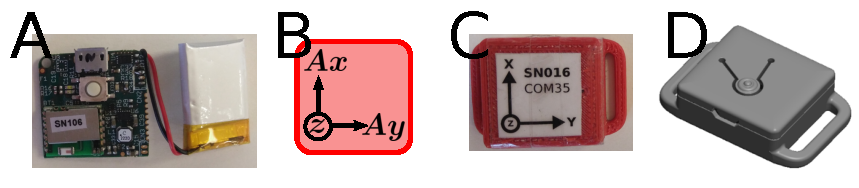
\includegraphics[width=0.9\textwidth]{muse}
   \caption
	[Inertial Measurament Sensor]{
	{\bf Inertial Measurement Sensor}
		(A) Printed Circuit Board (PCB) with 165mAh battery,
		(B) axis orientation, 
		(C) real case, and 
		(D) 3D model for the case.
}
   \label{fig:muse}
\end{figure}
%%---------------------------------(FIGURE)-------------------------------------

\subsection{Issues with IMUs} \label{appendix:imus:issues}
For the experiment of human-image imitation activities where eight activities 
were performed per participant, it has been observed that time 
synchronisation had issues because of the drift in time for time series data
(2 minutes of data collection).
Additionally, these experiments
had problems with disconnections to bluetooth module. 
In contrast, for the human-humanoid imitation activities
where only four activities were performed per participant 
(1 minutes of data collection), 
data collection of time series had fewer issues with regard 
to the drift in time and bluetooth data streaming.  


\section{Time-series preprocessing} \label{appendix:b:tps}

The following sections explain how the 
organising data in multidimensional arrays,
data synchronisation, data Synchronisation, and 
time alignment are computed. 
Code and data for the following sections is available at
\codelink{https://github.com/mxochicale/phd-thesis/tree/master/0_code_data/1_code/5_creation_of_curated_timeseries/code_raw2aligned}.

\subsection{Organising Data in Multidimensional Arrays}
Scripts in \MATLAB were created to synchronise the data using the clock 
drift and clock offset values which were provided for each of the 
NeMEMSi sensors. Then the data from each sensor is aligned in 
time using using \texttt{finddelay()} and \texttt{alignsignals()}.

\subsection{Data Synchronisation}
To find the delay between two two sensors that were attached to the same place
of the body parts, a function called  \texttt{finddelayMX()} was created.
Such function computes the autocorrelation between two signals using 
\texttt(xcorr())
then the maximum value of the autocorrleation function is extracted
to create a delay between the values of maximum index in the autocorrelation
function and the length of the first signal.
% [R, lag] = xcorr(X,Y);
% [Y,I] = max(R);  %%%[Y,I] = max(X) returns the indices of the maximum values in vector I.
% delay = abs(I - length( X ) );

The function \texttt{alignsignalsMX()} was used to align two signals based
on \texttt{finddelayMX()}. The function \texttt{alignsignalsMX()} use six inputs
of which sA and sB are for the sensors, windowframe for the information
of the signal is extracted from another activities, 
the MainAxis of which the signal are going to be extracted, 
the truncate delay that is created to
synchronise the signals adding an extra delay that is based on the length of
previous signals 
and tuning delay that can be useful to tune the delay in the
case of the delay is not appropriate when the signals are too noisy.
% function [a,b,delay] =
% alignsignalsMX(sA,sB,windowframe,MainAxis,truncate_delay, tuning_delay)
Then, \texttt{aligntwosignals()} is applied to align only two signals.
The inputs of \texttt{aligntwosignals()} are X and Y for the input vectors,
truncate delay for the previous delay of two signals and tuning delay
in case that signals are two noise and the xcorr fail to find an appropriate
delay.
 % function [a,b,delay] = aligntwosignals(X,Y,truncate_delay, tuning_delay)

\subsection{Time Alignment}
%It was taken another approach to align the data in time in which the
%original synchronised data is manipulated. 
Given four vectors of time
$t_1, t_2, t_3, t_4$, the minimum and maximum values were extracted 
for the start time of the four sequence of time,
it was also extracted the minimum and maximum values to the
end of each of the four sequences of time.
However, after aligning the vectors it has then  been noticed that there were
different values of length across vectors i.e., $1880,1986,1987,1988$.
Therefore the length for the second vector was used as the primary length
because is the one that presents the minimum value of the three maximum
lengths. Then \texttt{interp1(x,v,vq,'phchip')}  was used to interpolate the
length of each of the vectors, for example: $1986,1986,1986,1986$.
It has been chosen \texttt{phchip} function since the interpolation present
values for each of the points as oppose to \texttt{linear} function
which create NA values.


\newpage
\section{NAO -- humanoid robot}  \label{appendix:nao}
A NAO humanoid robot version 04 from SoftBank (Fig. \ref{fig:nao})
was used for the experiments of human-humanoid interaction. 
NAO were programmed for simple horizontal and vertical arm movements
using Choregraphe, an API to program NAO, and then 
interpolated values of the animation were exported 
to a python script.
%%---------------------------------(FIGURE)-------------------------------------
\begin{figure}[h]
 \centering
   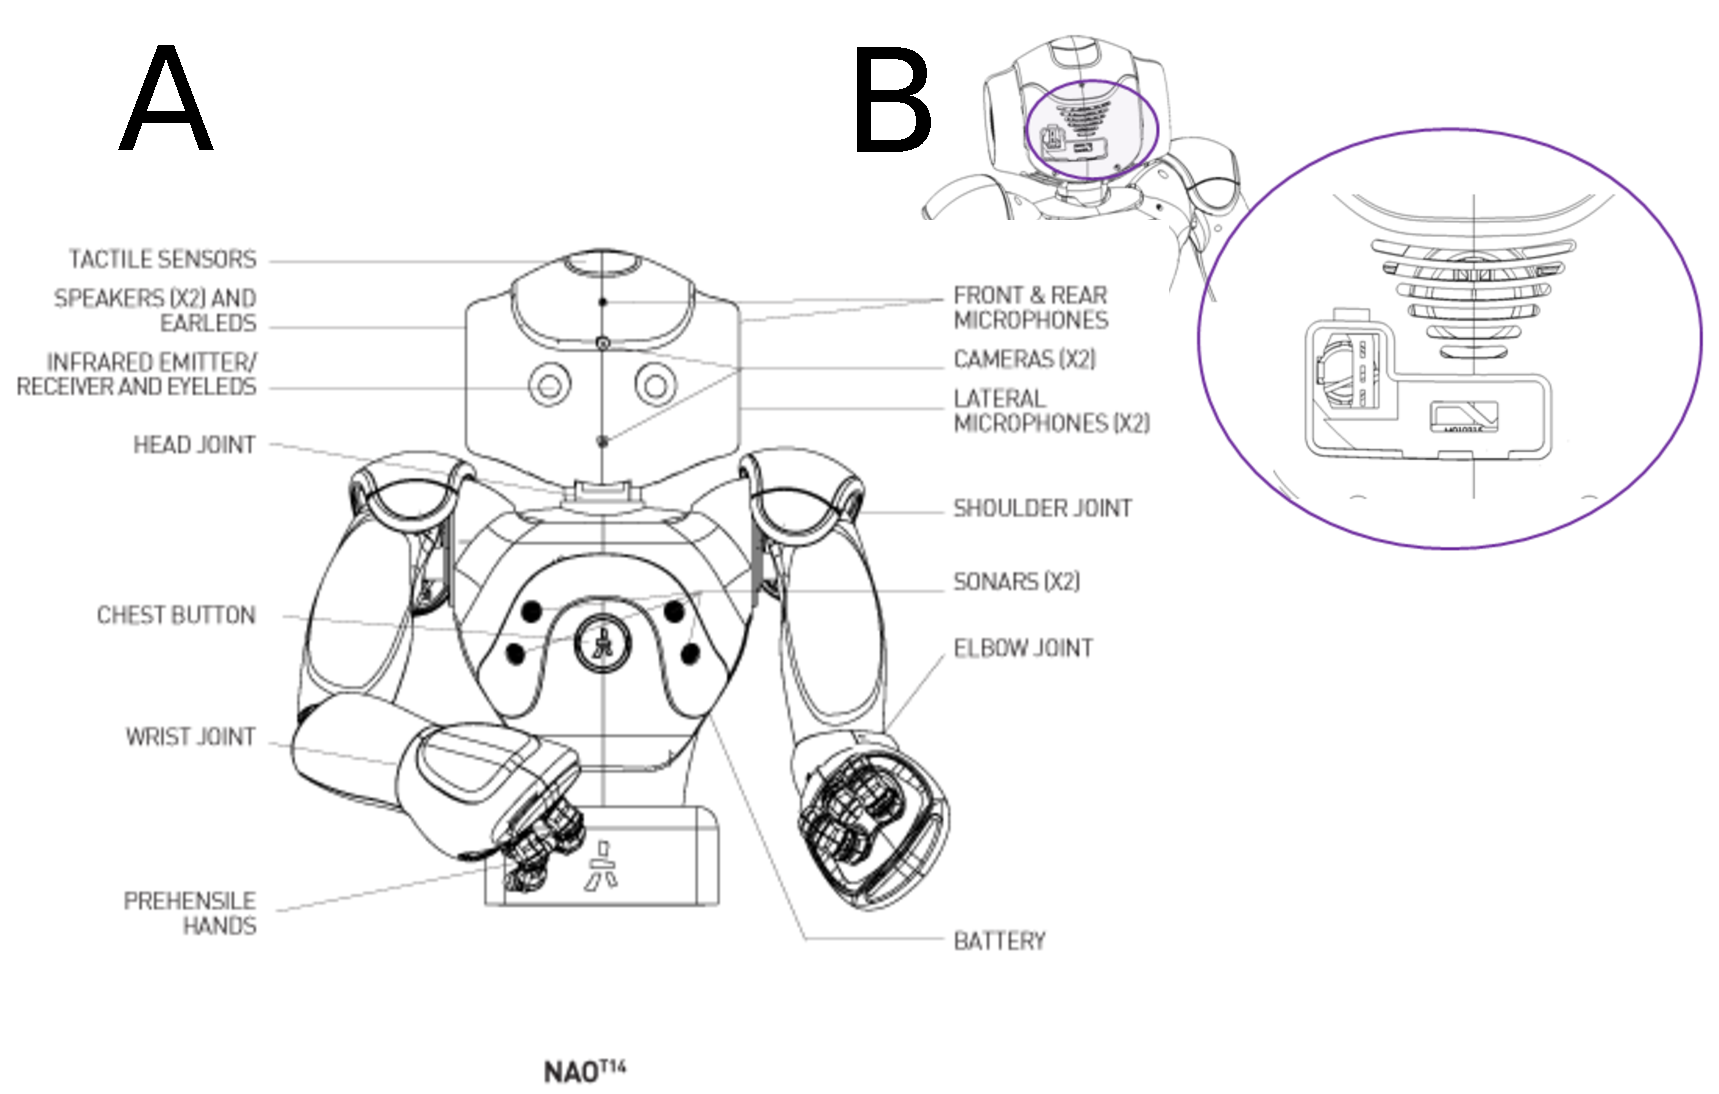
\includegraphics[width=1.0\textwidth]{nao}
   \caption
	[NAO, humanoid robot from SoftBank]{
	{\bf NAO, humanoid robot from SoftBank.}
		(A) NAO body type T4 with its parts, and 
		(B) back design of NAO version 04.
}
   \label{fig:nao}
\end{figure}
%%---------------------------------(FIGURE)-------------------------------------

